\chapter{本提案手法の実装}\label{cha:Implementation}
本提案手法は、領域座標取得部、文字情報取得部、ラベル付与部、ファイル出力部の4つの処理部で構成する。
本提案手法の構成を、図\ref{fig:structure}に示す。

以降、本章では4つの処理部について説明する。

\begin{figure}[t]
    \begin{center}
        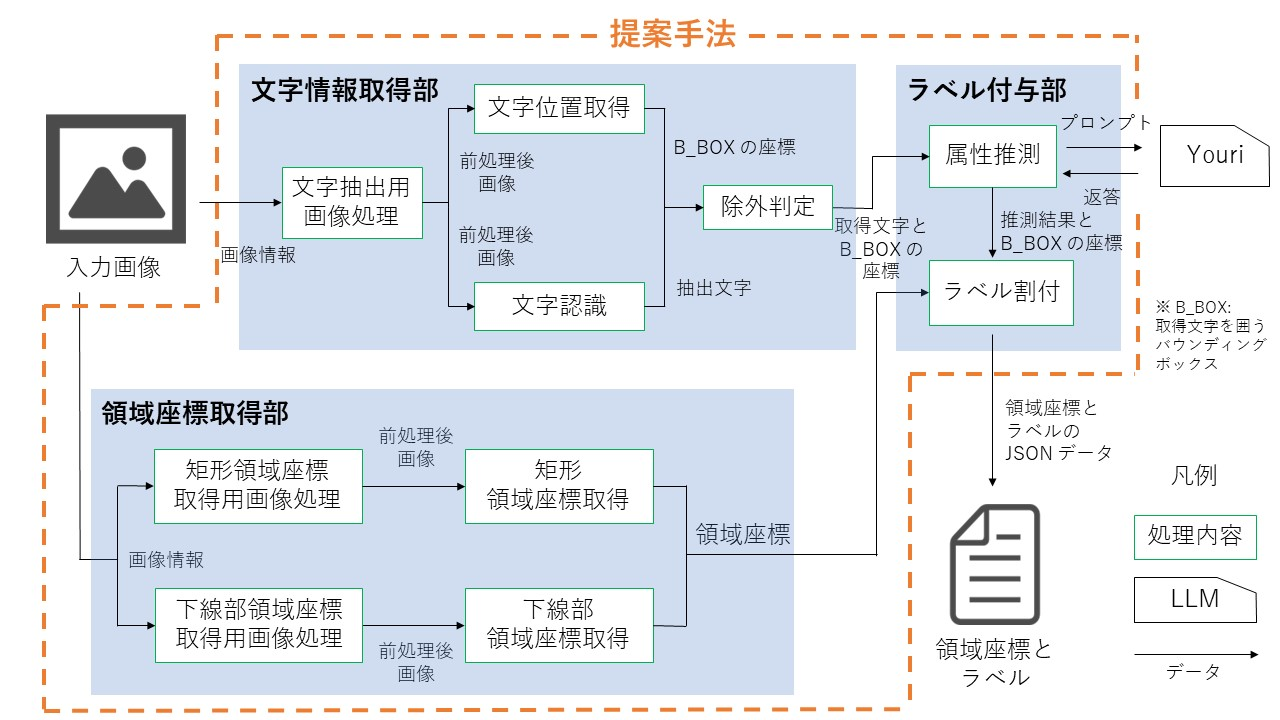
\includegraphics[width=15cm]{image/structure.jpg}
        \caption{本提案手法の構造}
        \label{fig:structure}
    \end{center}
\end{figure}


\section{領域座標取得部}\label{sec:area_coords_obtainment_part}
領域座標取得部は、帳票画像内にある記入欄を検出し、取得した座標を領域座標として出力する。
矩形の帳票画像記入欄については、各頂点のxy座標を、下線部の帳票画像記入欄については、両端点のxy座標を領域座標として取得する。
領域座標取得部の出力結果である領域座標は、ラベル付与部(\ref{subsec:label_link_processing}節で後述)で用いる。

\subsection{矩形領域座標取得用画像処理}\label{subsec:image_processing_for_rect_coords_obtainment}
矩形領域座標取得用画像処理は、矩形領域座標取得処理(\ref{subsec:rect_coords_obtainment_processing}節で後述)の実行にあたり、必要な画像処理を行う。
矩形の取得にあたり、OpenCVのfindContours関数(\ref{sec:OpenCV}節を参照)を用いる。
この関数を呼び出すとき、第一引数に渡す処理画像のパスについて、渡したパスの処理画像は白または黒色の画像でなければエラーが発生してしまうため、帳票画像に画像処理を施す必要がある。

以下に、矩形領域座標の取得に必要な画像処理の順を示す。

\begin{enumerate}
    \item OpenCVのcvtColor関数を用いた、帳票画像のグレースケール化
    \item DeblurGANv2(\ref{sec:DeblurGANv2}節を参照)の適用によるブレ除去後のグレースケール化帳票画像の生成\\
        DeblurGANv2を適用することにより、帳票画像を撮影する際に発生する画像内のブレを除去し、矩形の検出精度を高める。
    \item OpenCVのGaussianBlur関数(\ref{sec:OpenCV}節を参照)を用いた、ガウシアンフィルタによるノイズ除去\\
        本提案手法では、カーネルの縦幅と横幅を共に3、標準偏差を0とする。
    \item OpenCVのthreshold関数(\ref{sec:OpenCV}節を参照)を用いた、大津の二値化による二値画像への変換\\
        本提案手法では、閾値処理を大津の二値化として、閾値処理を決定する変数をTHRESH\_TOZERO\_INVに指定し、二値化する(\ref{sec:OpenCV}節を参照)。
        白黒を反転して二値化することにより、複数の矩形が隣接する場合に、それらを囲む矩形を不要に検出してしまうことを防ぐ。
    \item OpenCVのgetStructuringElement関数(\ref{sec:OpenCV}節を参照)を用いた、カーネルの作成\\
        本提案手法では、5行5列の矩形カーネルを作成する。
    \item OpenCVのdilate関数(\ref{sec:OpenCV}節を参照)を用いた膨張処理\\
        本提案手法では、getStructuringElement関数で作成した矩形カーネルを用いる。
        なお、膨張する回数は1回とする。
\end{enumerate}


\subsection{矩形領域座標取得処理}\label{subsec:rect_coords_obtainment_processing}
矩形領域座標取得処理は、矩形の記入欄を検出し、各頂点のxy座標を矩形領域座標として取得し、出力する処理である。
本処理の出力は、下線部領域座標取得処理(\ref{subsec:underline_coords_obtainment_processing}節)の一部で利用する。

\ref{subsec:image_processing_for_rect_coords_obtainment}節の画像処理後、OpenCVのfindContours関数(\ref{sec:OpenCV}節を参照)による輪郭検出を用いて矩形の帳票画像記入欄を検出し、矩形領域座標を取得する。
なお、以下の条件のいずれかに該当する矩形については、誤検知の可能性が高いとして、出力の対象外とする。

\begin{itemize}
    \item 面積が3000ピクセル以下である場合
    \item 一辺の長さが10ピクセル以下である場合
\end{itemize}



% スマートフォンのカメラで撮影する際にブレが生じた帳票画像を図\ref{fig:before_deblur}に示す。
% 図\ref{fig:before_deblur}に対して、DeblurGANv2を適用することによってブレを除去した画像を図\ref{fig:after_deblur}に示す。
% 図\ref{fig:before_deblur}と図\ref{fig:after_deblur}より、DeblurGANv2によるブレ除去によって、図\ref{fig:before_deblur}でブレている矩形の線が図\ref{fig:after_deblur}ではっきりとなっていることがわかる。

% \begin{figure}[t]
%     \centering
%     \begin{minipage}[t]{0.45\linewidth}
%       \centering
%       \fbox{
%         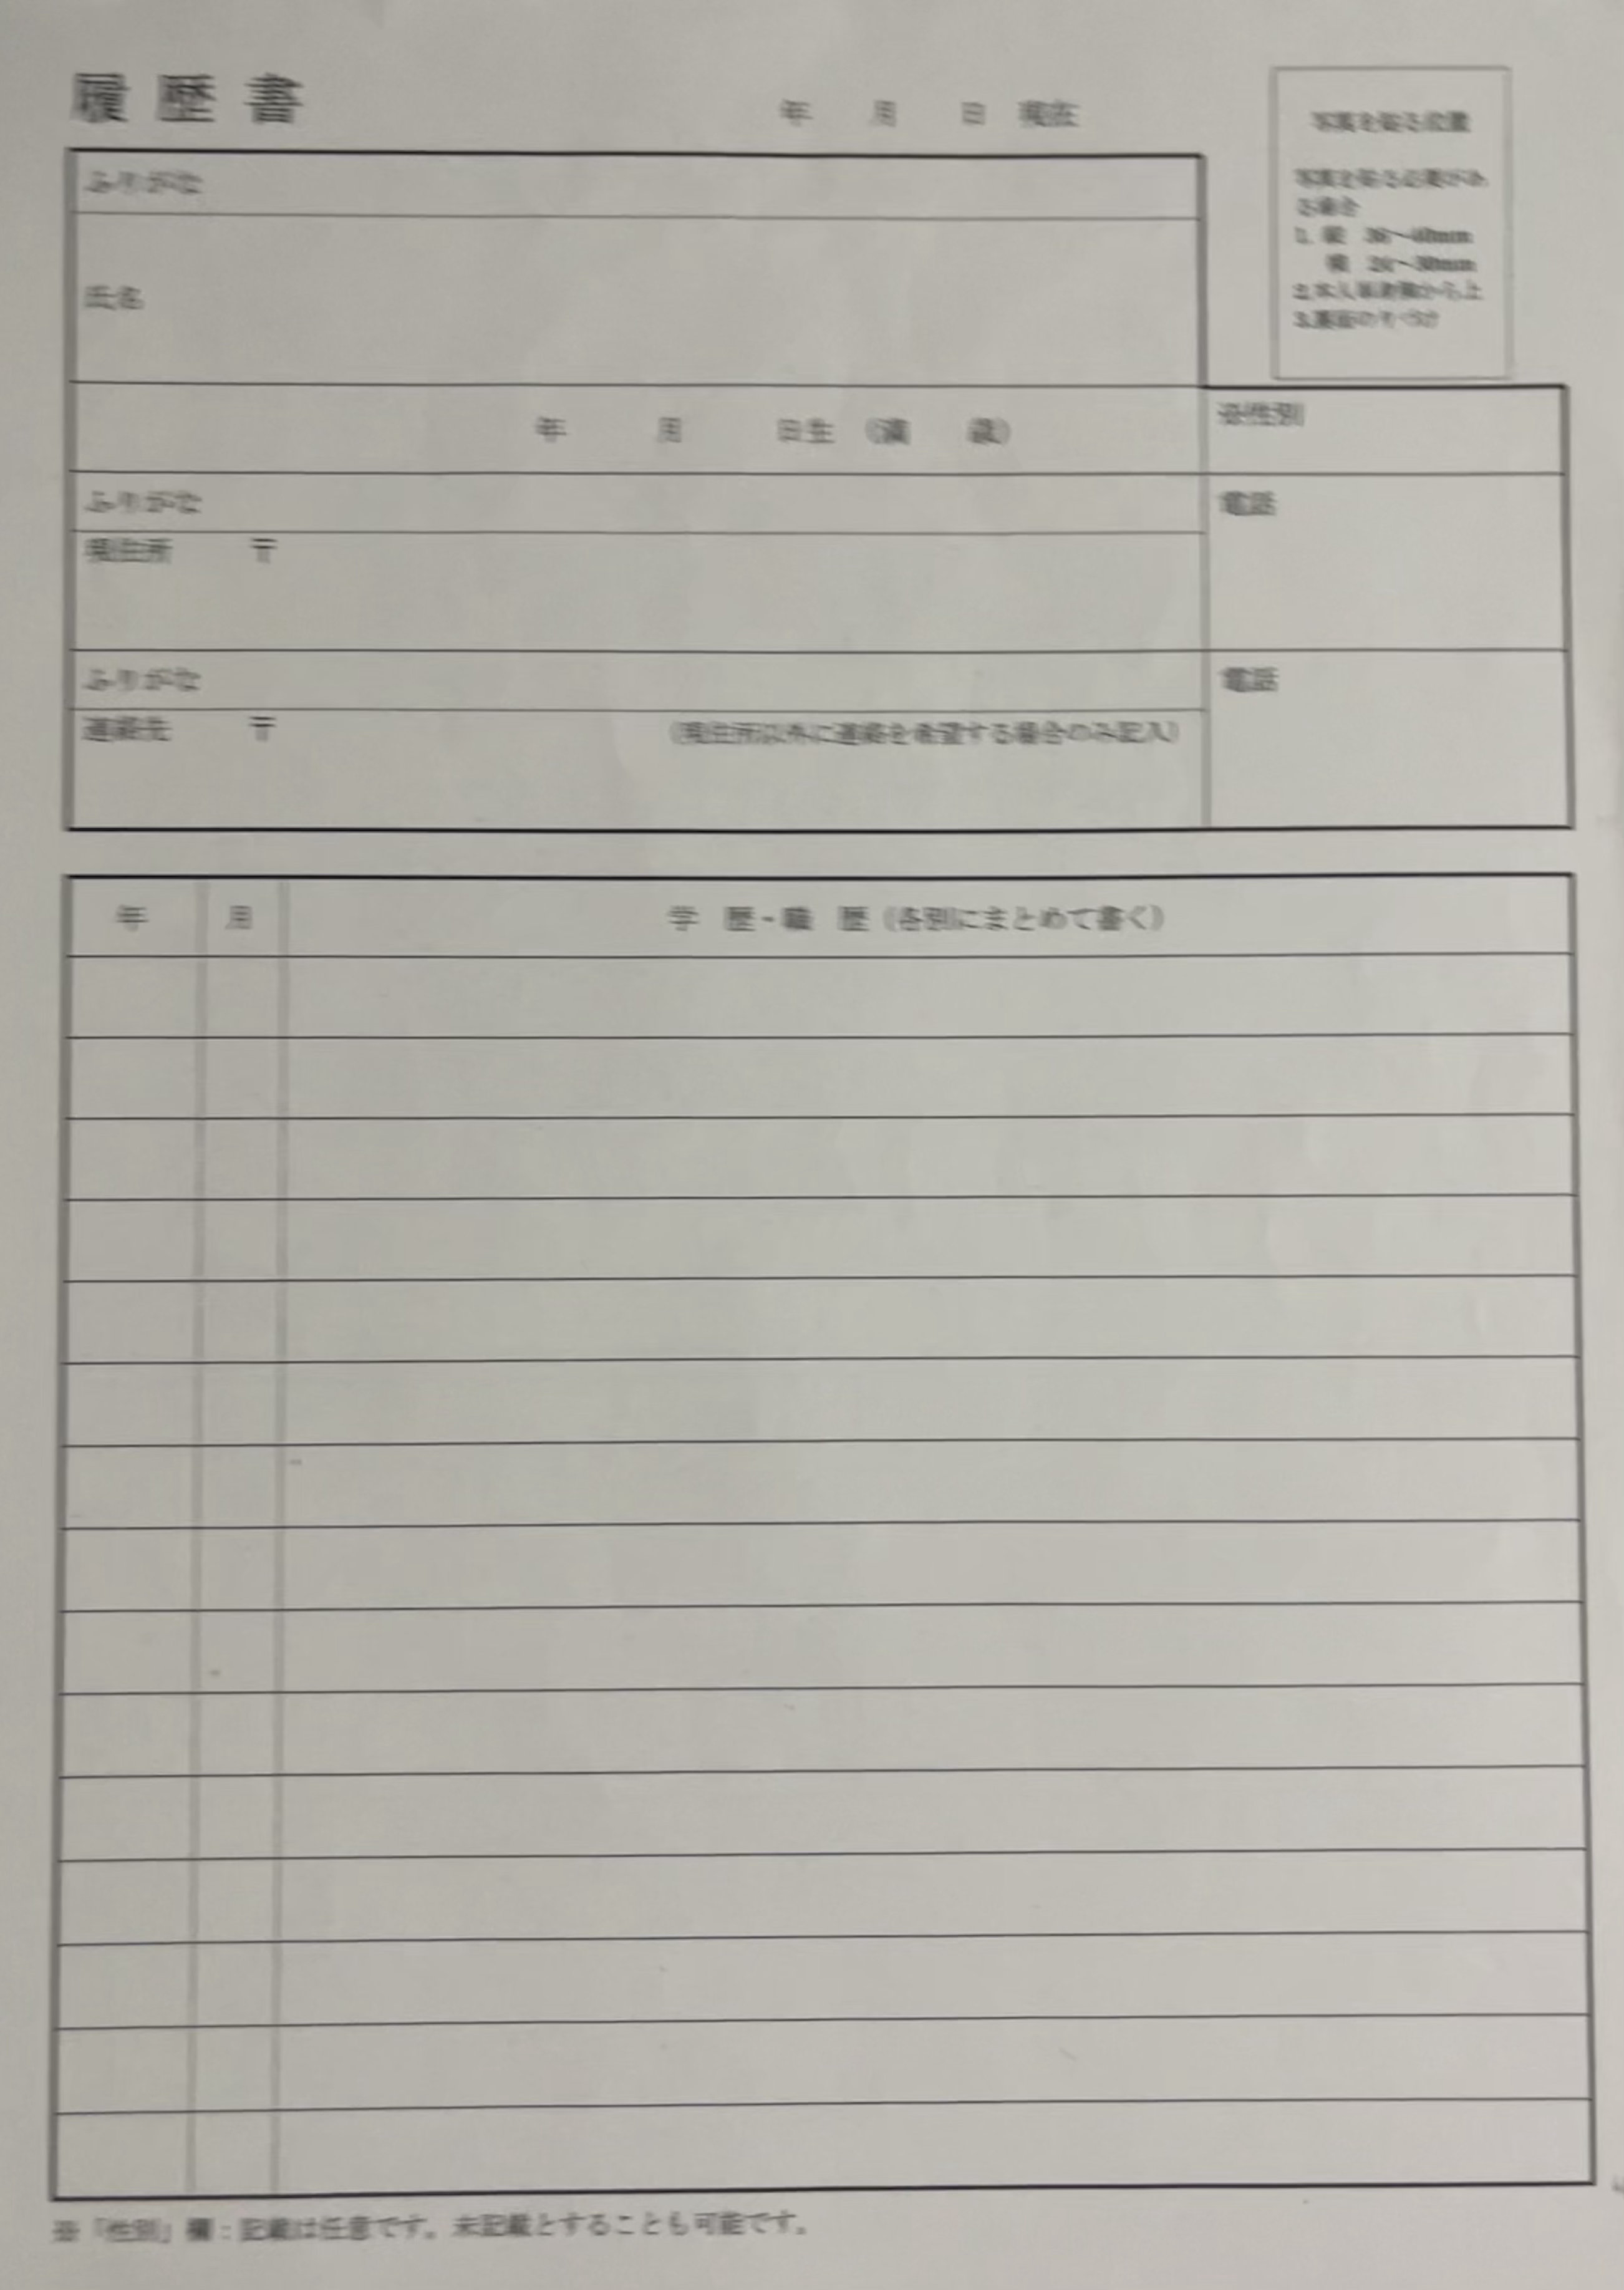
\includegraphics[keepaspectratio, width=7cm]{image/04-implementation/before_deblur.png}
%       }
%       \caption{撮影するにあたってブレが生じた帳票画像}
%       \label{fig:before_deblur}
%     \end{minipage}
%     \begin{minipage}[t]{0.45\linewidth}
%       \centering
%       \fbox{
%         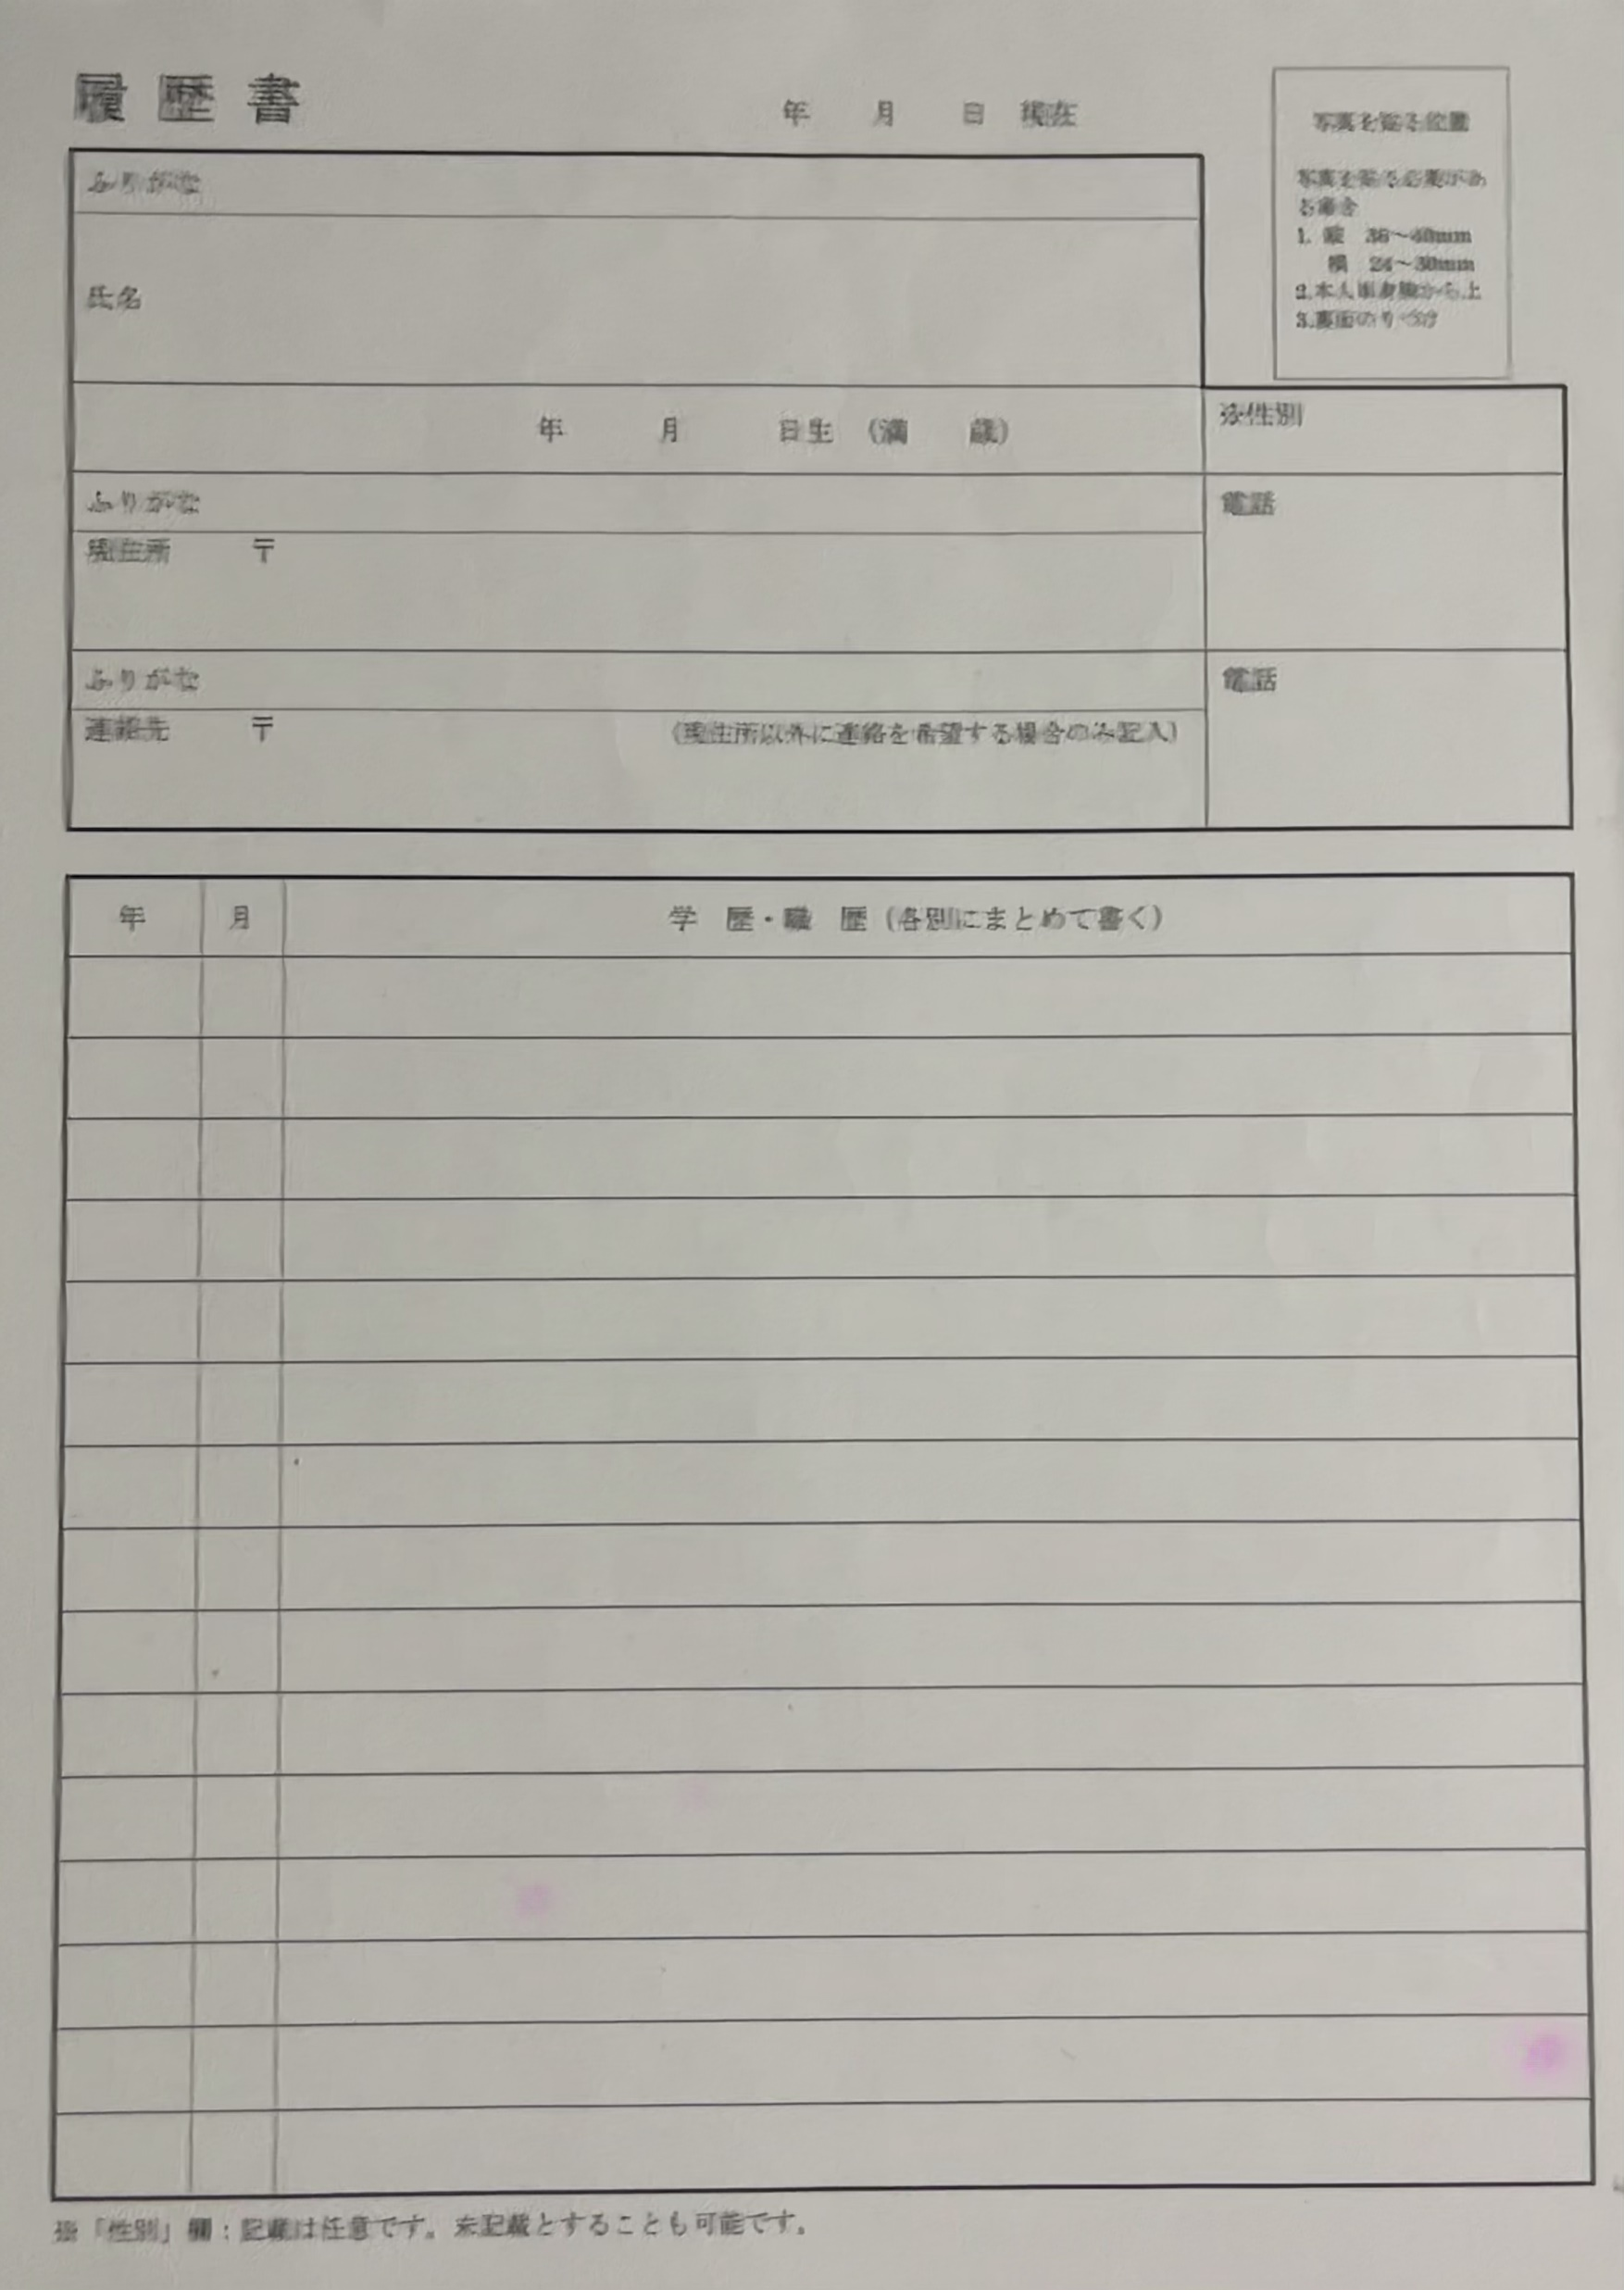
\includegraphics[keepaspectratio, width=7cm]{image/04-implementation/after_deblur.jpeg}
%       }
%       \caption{発生したブレを除去した帳票画像}
%       \label{fig:after_deblur}
%     \end{minipage}
% \end{figure}


\subsection{下線部領域座標取得用画像処理}\label{subsec:image_processing_for_underline_coords_obtainment}
下線部領域座標取得用画像処理は、下線部領域座標取得処理(\ref{subsec:underline_coords_obtainment_processing}節で後述)の実行にあたり、必要な画像処理を行う。
下線部の取得にあたり、OpenCVのHoughLinesP関数(\ref{sec:OpenCV}節を参照)を用いる。
この関数を呼び出すとき、第一引数に渡す処理画像のパスについて、渡すパスの処理画像は白または黒色の画像でなければエラーが発生してしまうため、帳票画像に画像処理を施す必要がある。

以下に、下線部領域座標の取得に必要な画像処理の順を示す。
なお、本処理における画像処理の一部は、矩形領域座標取得処理(\ref{subsec:rect_coords_obtainment_processing}節)と同様の画像処理を施す。

\begin{enumerate}
    \item OpenCVのcvtColor関数を用いた、帳票画像のグレースケール化\\
        \ref{subsec:rect_coords_obtainment_processing}節と同様の処理
    \item DeblurGANv2の適用によるブレ除去後のグレースケール化帳票画像の生成\\
        \ref{subsec:rect_coords_obtainment_processing}節と同様の処理
    \item OpenCVのthreshold関数を用いた、大津の二値化による二値画像への変換\\
        本提案手法では、閾値処理を大津の二値化として、閾値処理手法を決定する変数をTHRESH\_BINARY\_INVに指定し、二値化する。
        ハフ変換(同節で後述)は白線を検出する処理であるため、白黒を反転して二値化することにより、下線の検出精度を高める。
    \item OpenCVのthreshold関数(\ref{sec:OpenCV}節を参照)を用いた、Canny法によるエッジ検出\\
        本提案手法では、閾値処理における上限と下限の閾値を、以下のように決定する。
        \begin{enumerate}
            \item 大津の二値化で取得した閾値を受け取る。
            \item 中央値の定数倍(本研究では定数を0.33とする)を、取得した閾値から加減算する。
            \item 加算した値を上限の閾値、減算した値を下限の閾値として設定する。
        \end{enumerate}
\end{enumerate}


\subsection{下線部領域座標取得処理}\label{subsec:underline_coords_obtainment_processing}
下線部領域座標取得処理は、下線部の記入欄を検出し、両端点のxy座標を下線部領域座標として取得し、出力する処理である。

\ref{subsec:image_processing_for_underline_coords_obtainment}節の画像処理後、OpenCVのHoughLinesP関数によるハフ変換を用いて下線の帳票画像記入欄を検出し、下線部領域座標を取得する。
なお、以下の条件のいずれかに該当する直線については、誤検出の可能性が高いとして、出力の対象外とする。
条件の1つに矩形領域座標取得処理(\ref{subsec:rect_coords_obtainment_processing}節)の出力を利用する。

\begin{itemize}
    \item 直線の長さが10ピクセル未満である場合\\
        Canny法で適用するガウシアンフィルタで除去できていないノイズによって誤検出したエッジを下線と捉えることを防ぐ。
    \item 水平を基準として傾きが3ピクセル以上である場合\\
        横書きの帳票において、下線部の直線は水平であるため、垂直な直線を下線と捉えることを防ぐ。
    \item 直線が矩形領域の辺の一部から上下20ピクセル以内に存在する場合\\
        矩形領域座標取得処理の出力を利用する。矩形領域の辺の一部を下線と捉えることを防ぐ。
\end{itemize}

HoughLinesP関数によって直線を検出するとき、入力画像内にある1本の直線の上下に、誤って2本の直線を検出してしまう場合がある。
これは、両端点のxy座標が1ピクセル単位で異なる直線を、別の直線として検出するためである。
片方の端点が同じ場合は、傾きがある1本の直線として検出するが、両端点のxy座標が異なる場合は、上下に交差しない2本の別の直線として検出する。
これに対しては、検出した直線の中点を全て計算し、ある直線における中点のy座標について、上下10ピクセル以内に別の直線の中点が存在する場合は、二直線の両端点のxy座標をそれぞれ平均して1本の直線に統一することによって不具合を解消する。

\section{文字情報取得部}\label{sec:OCR_part}
文字情報取得部では、光学文字認識(\ref{sec:Optical-Charactor-Recognition}節を参照)によって、帳票画像内の文字についての情報を取得する。
本提案手法では、光学文字認識ソフトTesseract-OCRを用いて、文字と、文字を囲むバウンディングボックスの各頂点のxy座標を、それぞれ取得文字、文字位置として取得する。
文字情報取得部の出力結果は、ラベル付与部(\ref{subsec:label_link_processing}節で後述)で用いる。

\subsection{文字情報取得用画像処理}\label{subsec:image_processing_for_char_recognition}
文字情報取得用画像処理は、文字認識処理(\ref{subsec:char_recognition_processing}節で後述)および文字位置取得処理(\ref{subsec:char_position_obtainment_processing}節で後述)の処理にあたり、必要な画像処理を行う。
文字情報を取得するにあたって、文字の認識精度を高めるため、以下の順で帳票画像に画像処理を施す。

\begin{enumerate}
    \item DeblurGANv2の適用によるブレ除去後のグレースケール化帳票画像の生成\\
        \ref{subsec:rect_coords_obtainment_processing}節と同様の処理
    \item \ref{sec:area_coords_obtainment_part}節の出力である領域座標を取得\\
        後述する、領域を白色で描画する処理で利用するため。
    \item OpenCVのdrawContours関数(\ref{sec:OpenCV}節を参照)と、OpenCVのline関数(\ref{sec:OpenCV}節を参照)を用いた、白色で矩形領域と下線部領域の描画\\
        帳票画像に対して、矩形領域座標は矩形を、下線部領域座標は直線を白色で描画することによって、帳票画像記入欄を白くする。
        本提案手法では、白色かつ太さ15ピクセルの矩形と直線を描画する。
    \item OpenCVのimwrite関数を用いた、画像の保存\\
        画像を保存し、処理対象の画像を、入力である帳票画像から、白色で領域を描画した画像に変更する。
    \item OpenCVのcvtColor関数を用いた、帳票画像のグレースケール化\\
        \ref{subsec:rect_coords_obtainment_processing}節と同様の処理
    \item OpenCVのthreshold関数を用いた、大津の二値化による二値画像への変換\\
        本提案手法では、閾値処理を大津の二値化として、閾値処理を決定する変数をTHRESH\_BINARYに指定し、二値化する。
\end{enumerate}

矩形領域と下線部領域の白色で描画することによって、文字認識に不要な黒色の画素が白色となる。
これにより、文字認識に適切な閾値を計算することができるため、文字認識の精度が向上する。

\subsection{文字認識処理}\label{subsec:char_recognition_processing}
文字認識処理は、認識した文字を取得文字として取得する処理である。
\ref{subsec:image_processing_for_char_recognition}節の画像処理後、Tesseract-OCRによる文字認識を行う。
本提案手法では、PythonのOCR用のラッパーライブラリであるPyOCRから、変数builderにLineBoxBuilderを指定し、行単位で文字認識を行う。
文字認識処理と同時に、文字認識処理(\ref{subsec:char_recognition_processing}節)を行う。
変数builderにLineBoxBuilderを指定することで、行単位で文字認識と、文字位置を取得することができる。

\subsection{文字位置取得処理}\label{subsec:char_position_obtainment_processing}
文字位置取得処理は、認識した文字を囲むバウンディングボックスの各頂点のxy座標を文字位置として取得する処理である。
本処理は文字認識処理(\ref{subsec:char_recognition_processing}節)と同時に行い、文字位置を取得する。

文字位置取得後、バウンディングボックスの左上頂点のy座標を参照し、昇順にソートし、番号を0から順に割り振る。
y座標が同じ場合は、さらにx座標を参照し、昇順にソートする。
本来は、y座標が同じ場合は、x座標を昇順にソートするため、左から右へ番号が大きくなる。
しかし、人間の目視で複数の文字が同じ行に存在すると認識するとき、割り振った番号を参照すると、番号が入れ替わる不具合が発生する場合がある。
ラベル付与部(\ref{subsec:label_link_processing}節で後述)で文字位置を扱う際に、この不具合が起こった場合、ラベルの更新順が変化してしまい、意図しないラベルを領域座標に割り付ける可能性がある。

ある帳票画像に対して文字位置取得処理を施し、同行に存在する文字列に対して、割り振った番号が入れ替わったときの画像を、図\ref{fig:before_sorted_string}に示す。
図\ref{fig:before_sorted_string}内に描画している赤い矩形は、取得茂地を囲うバウンディングボックスであり、バウンディングボックスの左上頂点の上に、ソートしたときに割り振った番号を表示している。
図\ref{fig:before_sorted_string}内では、割り振った番号は、左から14番、15番、13番、12番となっている。
本来は、左から12番、13番、14番、15番となるよう並ぶ必要がある。

\begin{figure}[t]
    \begin{center}
        \fbox{
            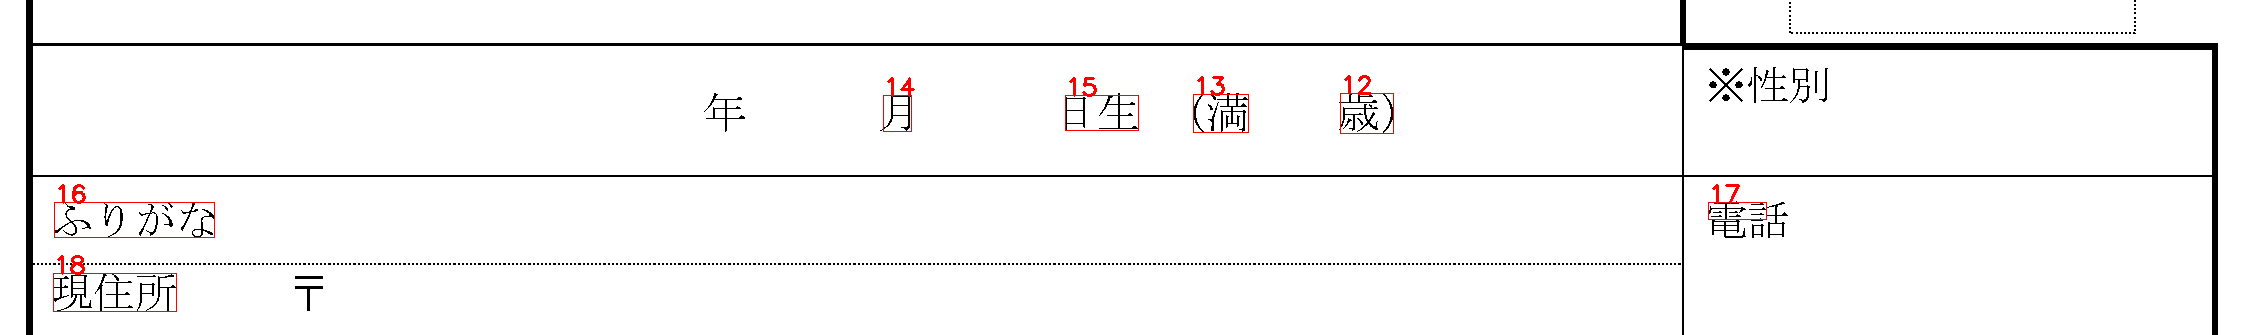
\includegraphics[width=15cm]{image/04-implementation/before_sorted_string.png}
        }
        \caption{誤って番号を割り振った文字位置}
        \label{fig:before_sorted_string}
    \end{center}
\end{figure}

これは、Tesseract-OCRが文字を認識する順番を、y座標についてピクセル単位で昇順にソートするため、人間の目視で認識する順番とソート後の順番に違いが生じるためである。
以下に、この不具合の発生を防ぐため、再ソートを行う流れを示す。
以下の処理は、文字を認識した順番で、iを0に初期化し、取得文字の数だけ繰り返す。

\begin{enumerate}
    \item i番目のバウンディングボックスの左上頂点のy座標を取得する。
    \item 取得したy座標を基準として、10ピクセル以内に別のバウンディングボックスの左上頂点が存在する場合は、以下の処理を行う。
    \begin{enumerate}
        \item 条件にあてはまる左上頂点のxy座標全てを、リストgroupに格納する。
        \item リストgroup内について、x座標を参照して再ソートする。
        \item iをgroupの要素数だけ増やす。
    \end{enumerate}
\end{enumerate}

これによって、人間の目視で同じ行に存在すると認識する複数の文字を対象に、文字位置取得時点のy座標について、最小のy座標と最大のy座標の差が10ピクセル以内であれば、正しくソートができる。
再ソートによって、番号を正しく並び替え、バウンディングボックスを描画した画像を図\ref{fig:after_sorted_string}に示す。
ソート後は、図\ref{fig:after_sorted_string}内における12番から15番は、左から12番、13番、14番、15番となっており、左右の順番を入れ替えることに成功していることがわかる。

\begin{figure}[t]
    \begin{center}
        \fbox{
            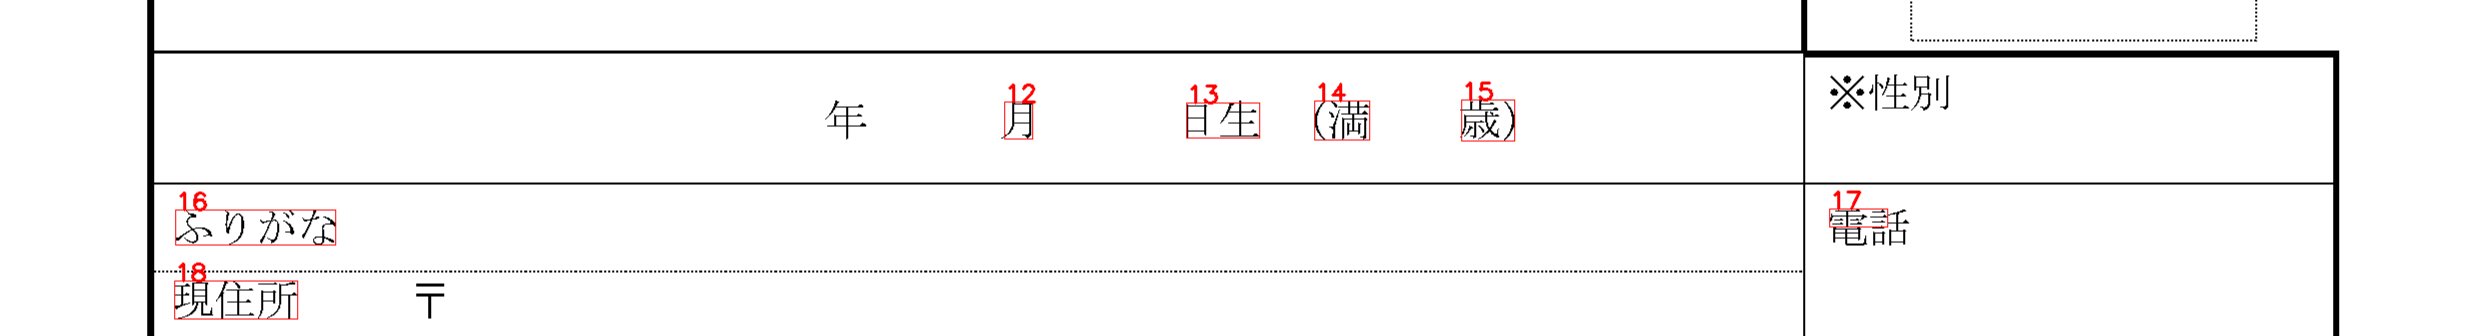
\includegraphics[width=15cm]{image/04-implementation/after_sorted_string.png}
        }
        \caption{同行の番号を左から右へ昇順となるようソートした文字位置}
        \label{fig:after_sorted_string}
    \end{center}
\end{figure}

図\ref{fig:original}に示した帳票画像に対して、文字認識処理と文字位置取得処理を行った結果を、図\ref{fig:char_recognition_for_original}に示す。
また、図\ref{fig:char_recognition_for_original}で示す文字位置を参照し、バウンディングボックスを描画した画像を、図\ref{fig:bbox_recognition_for_original}に示す。
図\ref{fig:char_recognition_for_original}は、以下の順で、取得文字と文字位置を表す。

\begin{enumerate}
    \item \ref{subsec:char_position_obtainment_processing}節で割り振った、ソート後の番号
    \item バウンディングボックスの左上頂点のxy座標
    \item バウンディングボックスの右下頂点のxy座標
    \item 取得文字
\end{enumerate}

例えば、番号1の取得文字は、「請求日」であり、バウンディングボックスの左上頂点のxy座標が、(1597, 321)であり、バウンディングボックスの右下頂点のxy座標が、(1724, 363)となる。
図\ref{fig:char_recognition_for_original}の番号は、図\ref{fig:bbox_recognition_for_original}のバウンディングボックスの左上頂点の上に表示する番号と一致する。

\lstset{language=}
\begin{figure}[t]
    \begin{lstlisting}
    string[0] ((1644, 244), (1730, 285)) : 番号
    string[1] ((1597, 321), (1724, 363)) : 請求日
    string[2] ((1343, 486), (1411, 528)) : 詩
    string[3] ((1046, 518), (1106, 555)) : 月
    string[4] ((1194, 487), (1260, 555)) : 求
    string[5] ((1354, 530), (1400, 555)) : 較
    string[6] ((898, 683), (983, 725)) : 御中
    string[7] ((223, 992), (926, 1034)) : 下記の通り、ご請求申し上げます。
    string[8] ((1573, 1073), (1662, 1106)) : FAX
    string[9] ((229, 1147), (449, 1189)) : ご請求金額
    string[10] ((1126, 1147), (1248, 1190)) : (税込)
    string[11] ((1574, 1146), (1656, 1187)) : 担当
    string[12] ((1183, 1313), (1270, 1354)) : 数量
    string[13] ((1526, 1311), (1606, 1352)) : 単価
    string[14] ((1970, 1311), (2058, 1352)) : 合計
    string[15] ((1521, 2267), (1608, 2308)) : 小計
    string[16] ((1499, 2343), (1632, 2386)) : 消費税
    string[17] ((1520, 2422), (1608, 2463)) : 合計
    string[18] ((1160, 2576), (1293, 2619)) : 備考
    \end{lstlisting}
    \caption{図\ref{fig:original}から取得した文字}
    \label{fig:char_recognition_for_original}
\end{figure}

\begin{figure}[t]
    \begin{center}
        \fbox{
            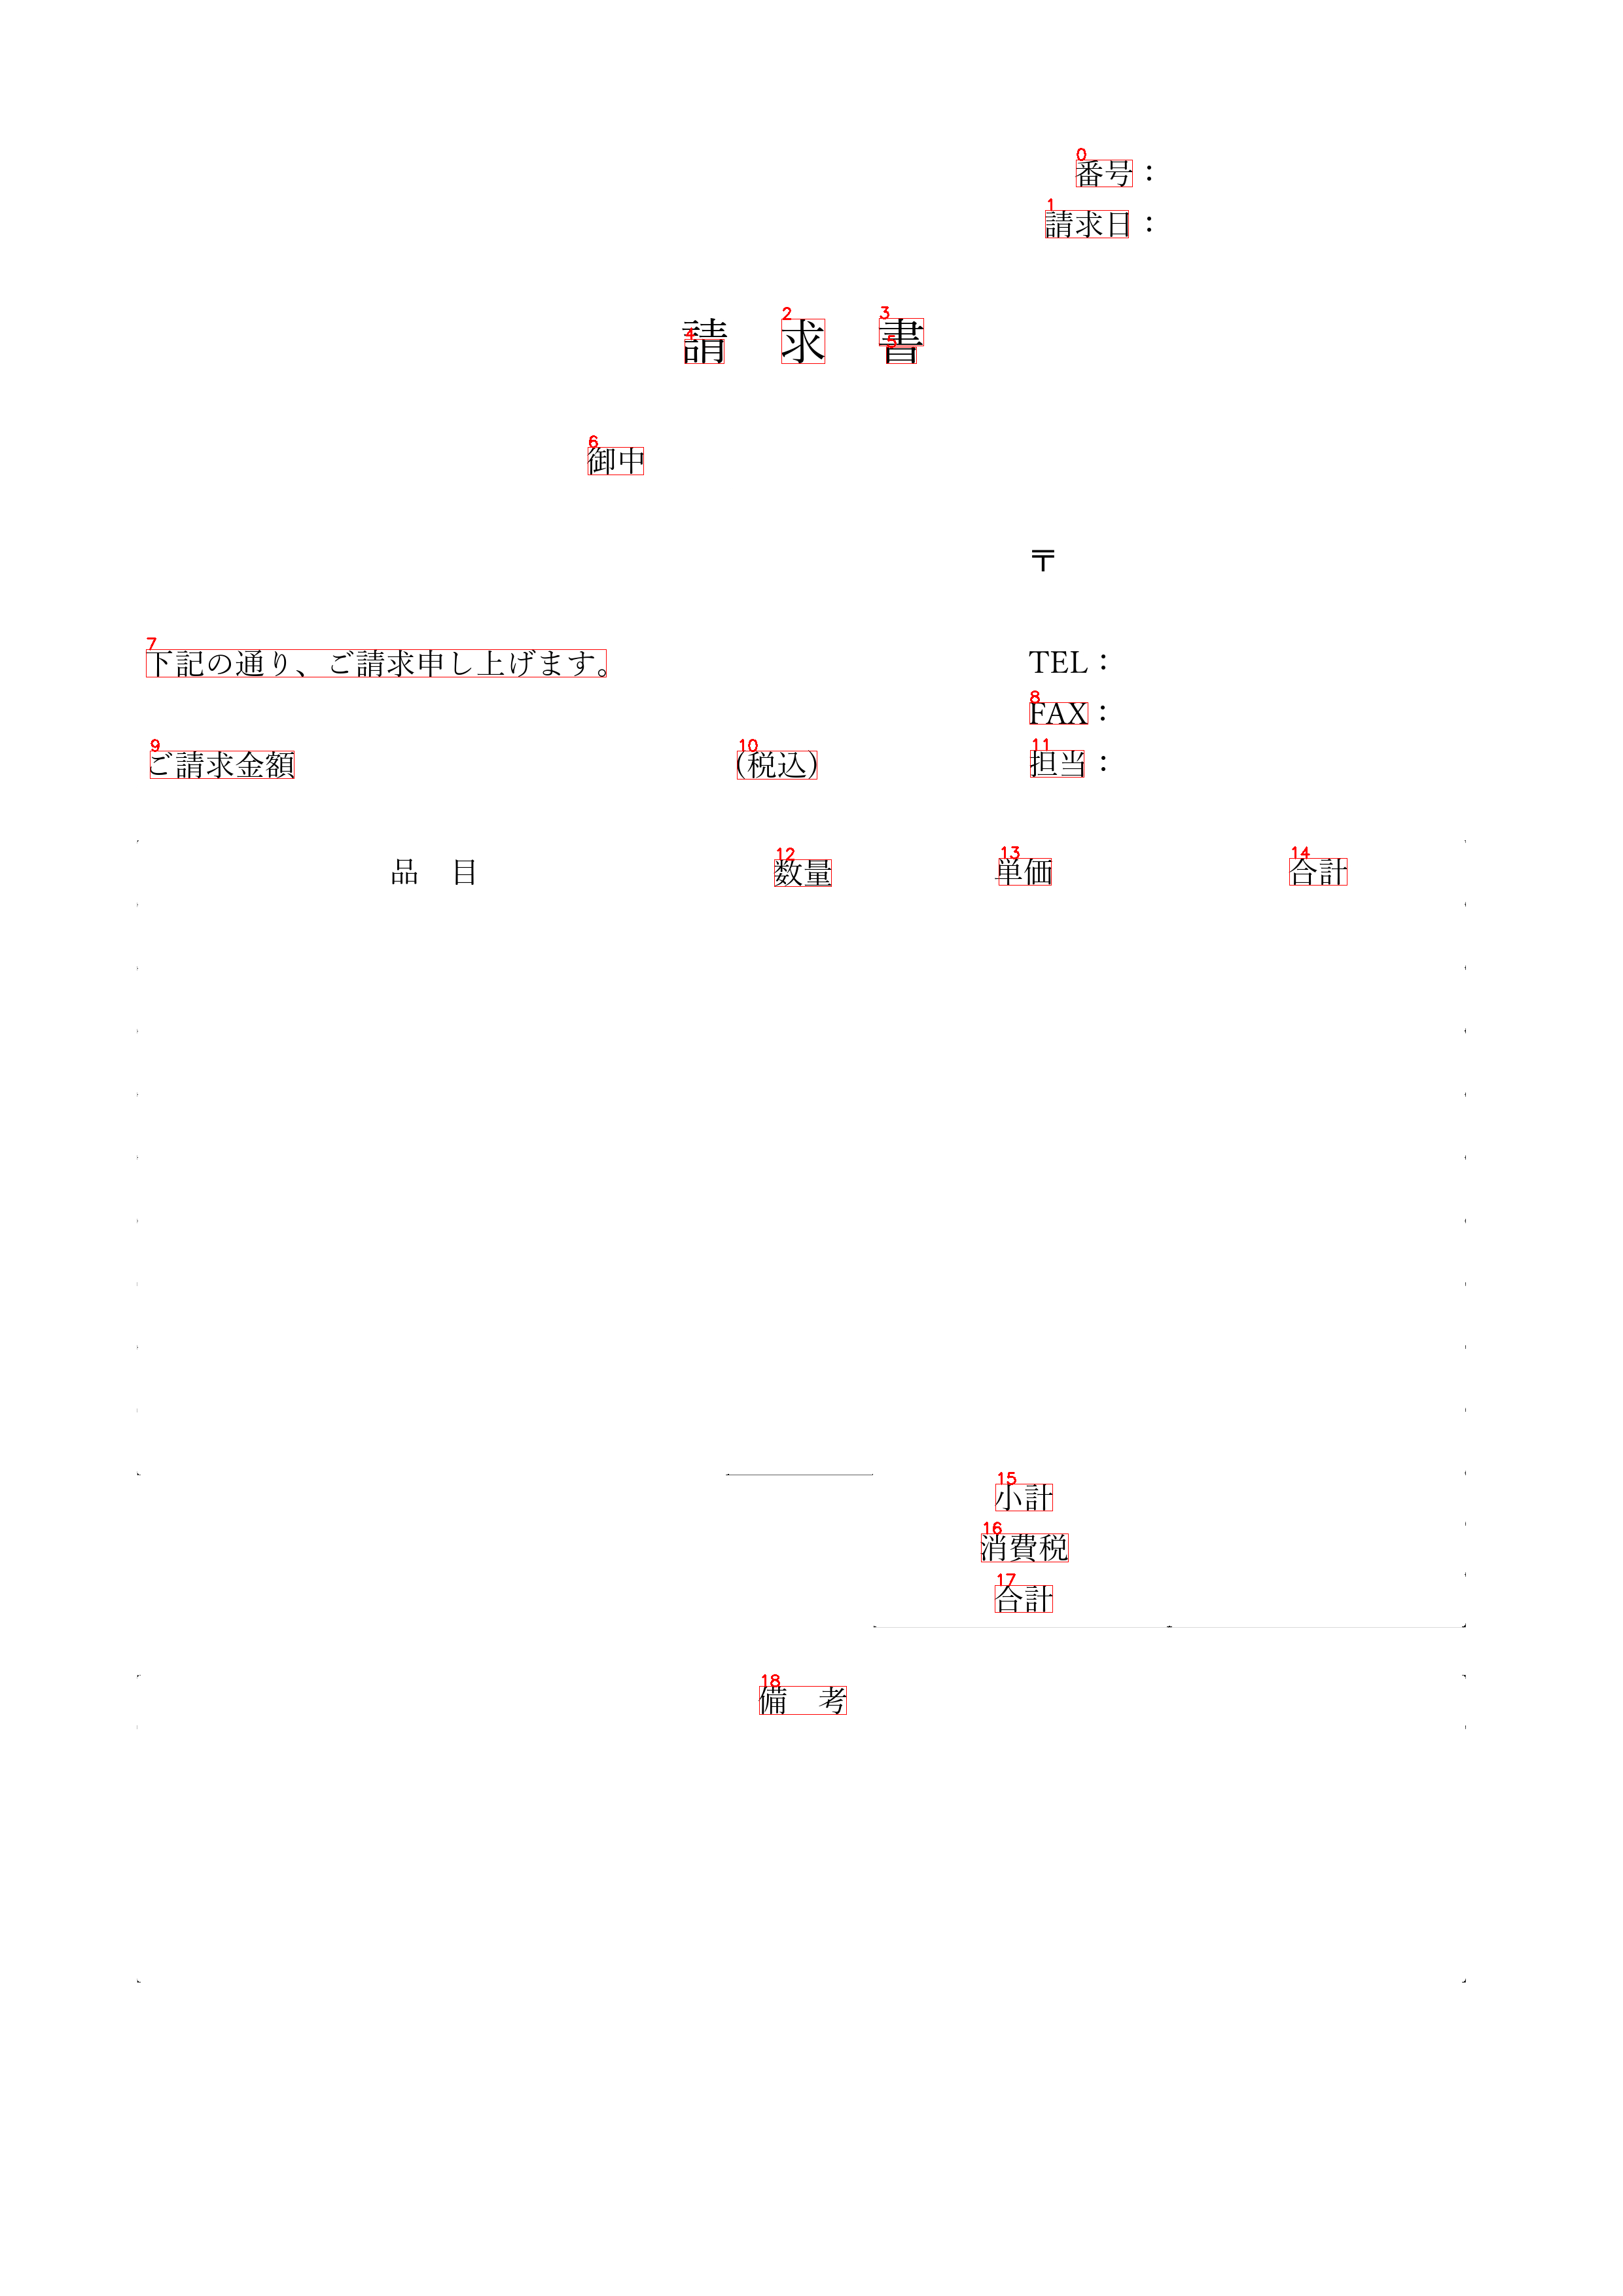
\includegraphics[width=15cm]{image/04-implementation/char_with_bbox.png}
        }
        \caption{図\ref{fig:char_recognition_for_original}の文字位置を図\ref{fig:original}の画像に描画した画像}
        \label{fig:bbox_recognition_for_original}
    \end{center}
\end{figure}

\subsection{除外判定処理}\label{subsec:exclusion_judgement_processing}
除外判定処理は、Fugashi(\ref{sec:Fugashi}節を参照)による形態素解析を行い、属性判定処理(\ref{subsec:att_prediction_processing}節で後述)に不要である取得文字について、出力から除外する処理である。
日本語の文章は、英語の文章のように、単語が形態素ごとにスペースで区切られていないため、\ref{subsec:char_and_bbox_obtainment}で得た取得文字のままでは、形態素への分割および品詞の解析が難しい。
そこで、形態素解析ソフトウェアであるMecab(\ref{sec:Fugashi}節を参照)を用いて、取得文字を形態素に分割し、品詞を解析する。
形態素の品詞を解析し、取得文字の構成形態素数のうち、特定の品詞である形態素数の割合が半分以上である場合は、属性判定において意味がない取得文字であるとして、該当の取得文字と文字位置を文字情報取得部の出力から除外する。
文字を認識する際に、紙面と背景の境界や、矩形や直線を文字として誤認識する場合がある。
不要な文字の属性推測処理を防ぐことにより、処理時間を短縮することができる。

以下に、UniDic品詞体系(左からカンマ区切りで、大分類、中分類、小分類、細分類)をもとに、除外対象である形態素の品詞を示す。
なお、除外対象とする品詞は、経験から決定している。

\begin{itemize}
    \item 補助記号,一般,*,*
    \item 感動詞,一般,*,*
    \item 感動詞,フィラー,*,*
\end{itemize}

ある帳票画像に対して、認識した文字のバウンディングボックスを描画した画像の一部を、図\ref{fig:before_exclusion_bbox}に示す。
また、図\ref{fig:before_exclusion_bbox}で描画したバウンディングボックスに対応する取得文字を出力した画像を、図\ref{fig:before_exclusion_string}に示す。
図\ref{fig:before_exclusion_bbox}、図\ref{fig:before_exclusion_string}内の58番および60番は、帳票画像内の矩形の辺を誤って文字として認識している。
この矩形については、文字情報取得用画像処理(\ref{subsec:image_processing_for_char_recognition}節)で取得できなかったため、白い矩形を描画できていない。
図\ref{fig:before_exclusion_bbox}、図\ref{fig:before_exclusion_string}内の58番および60番の取得文字は、属性推測処理において意味がない文字である。
図\ref{fig:before_exclusion_string}に示した取得文字に対して除外判定処理を適用し、属性推測処理に不要な取得文字を除外した出力を、図\ref{fig:after_exclusion_string}に示す。
図\ref{fig:after_exclusion_string}より、属性推測処理に不要な取得文字の除外に成功していることがわかる。

\begin{figure}[t]
    \begin{center}
        \fbox{
            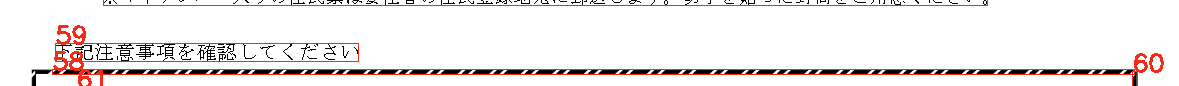
\includegraphics[width=15cm]{image/04-implementation/before_exclusion_bbox.png}
        }
        \caption{属性判定に不要な文字を含む文字認識}
        \label{fig:before_exclusion_bbox}
    \end{center}
\end{figure}

\begin{figure}[t]
    \begin{center}
        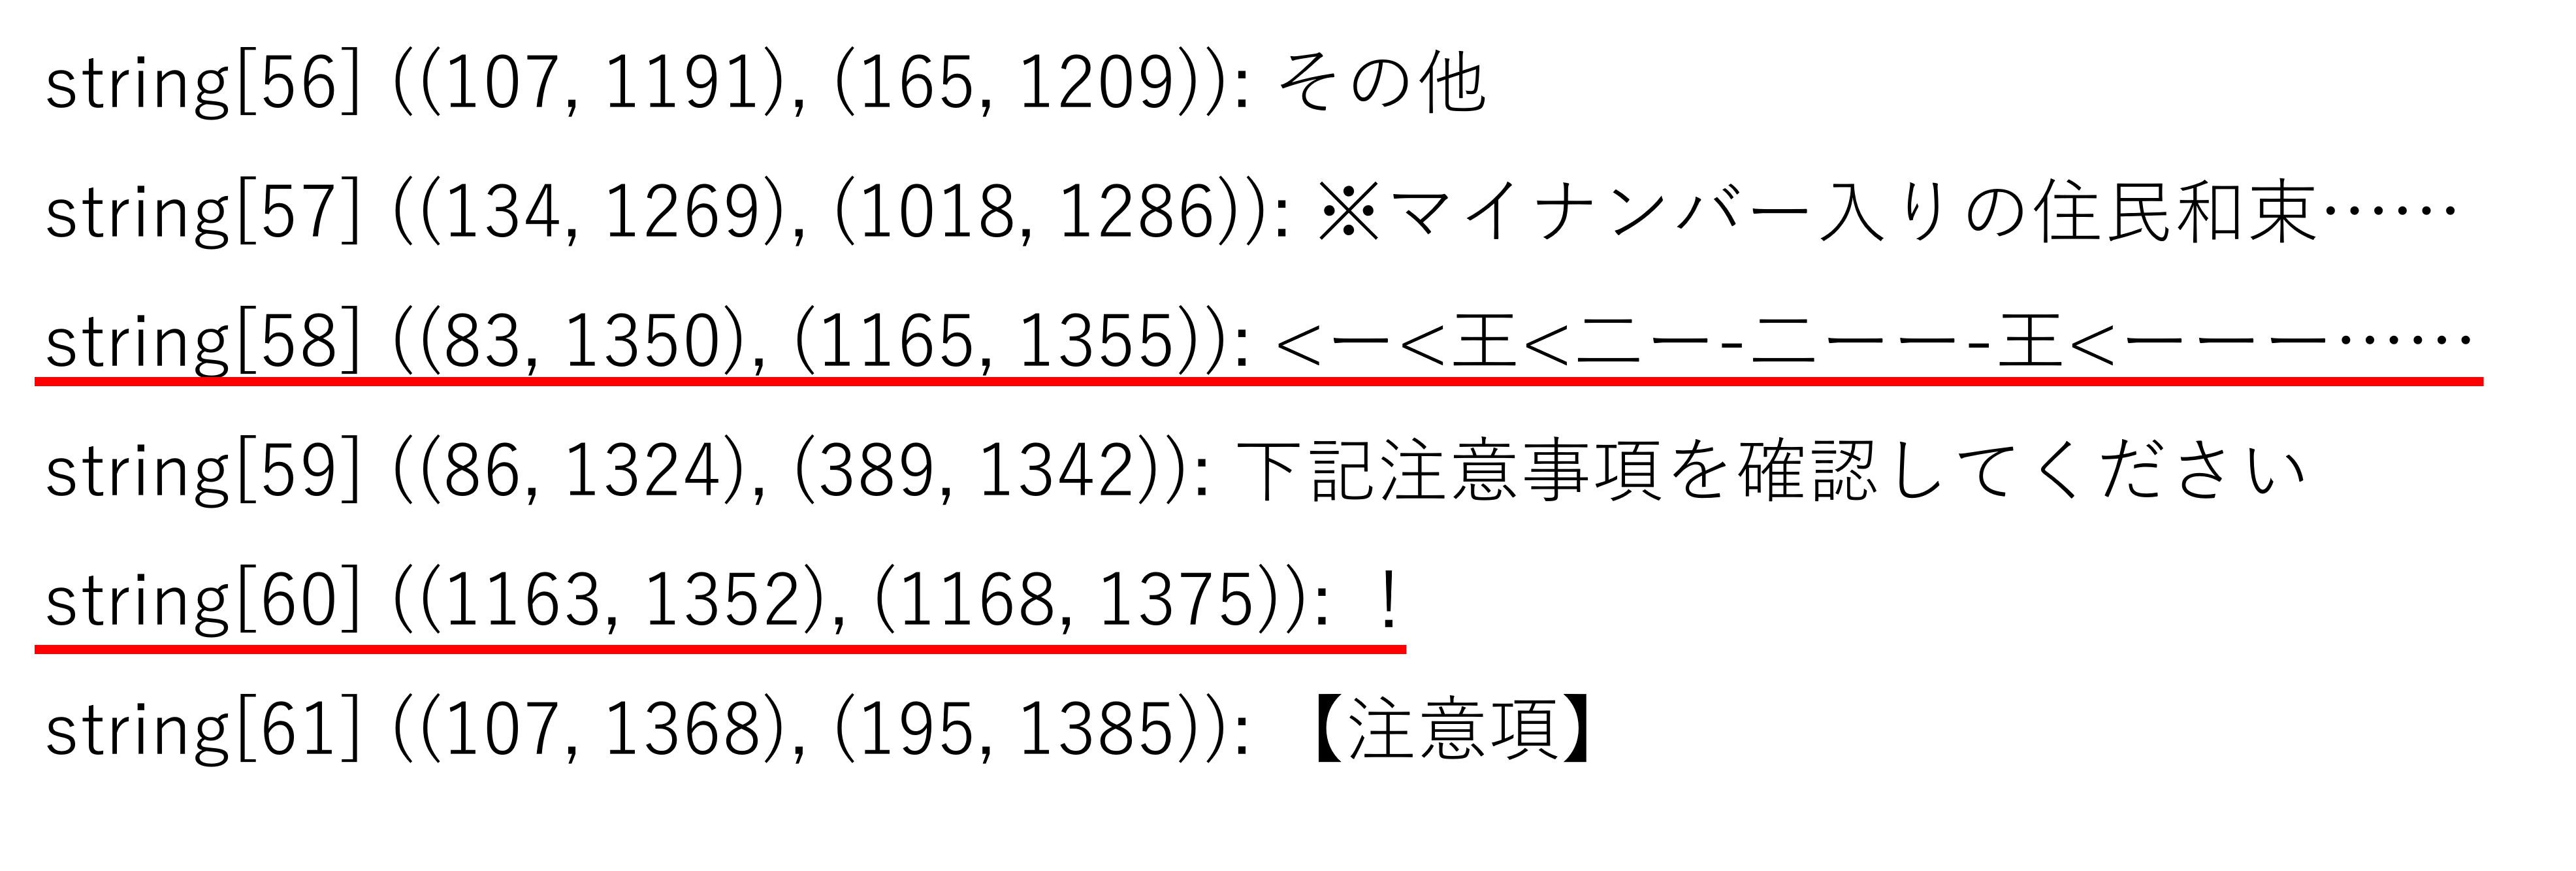
\includegraphics[width=15cm]{image/04-implementation/before_exclusion_string.png}
        \caption{除外判定処理適用前の取得文字}
        \label{fig:before_exclusion_string}
    \end{center}
\end{figure}

\begin{figure}[t]
    \begin{center}
        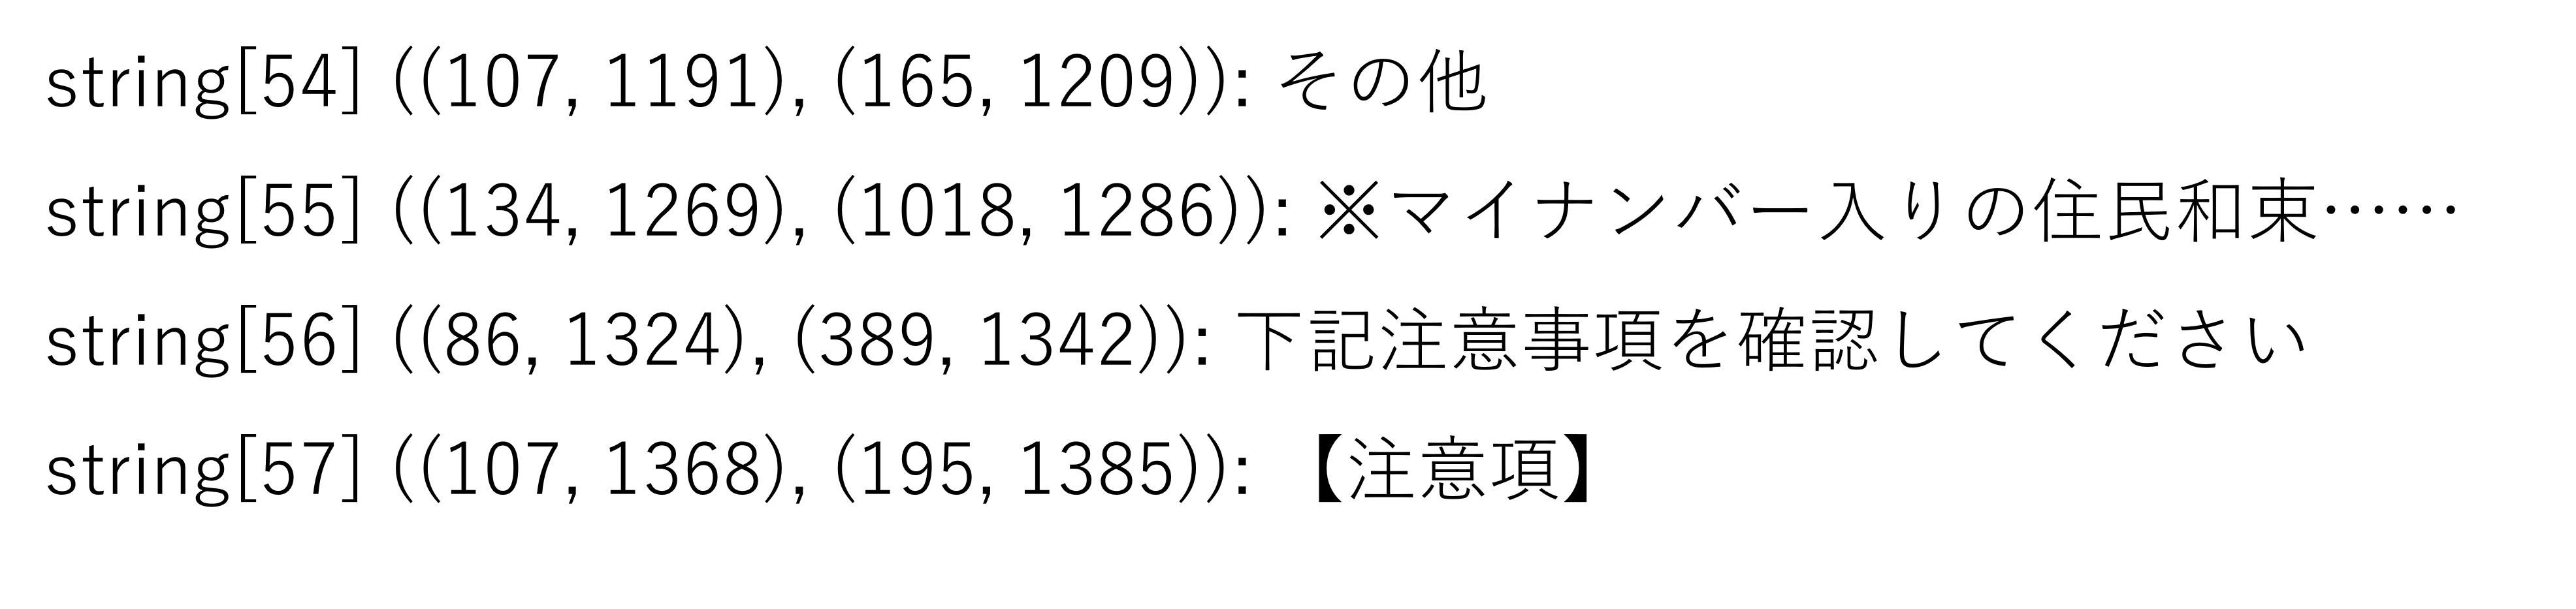
\includegraphics[width=15cm]{image/04-implementation/after_exclusion_string.png}
        \caption{除外判定処理適用後の取得文字}
        \label{fig:after_exclusion_string}
    \end{center}
\end{figure}

\section{ラベル付与部}\label{sec:label_link_part}
ラベル付与部では、除外判定処理(\ref{subsec:exclusion_judgement_processing}節)後の取得文字の属性を、属性の候補(\ref{subsec:att_prediction}節を参照)である、日付(date)、文字列(string)、数値(number)の3つから適切な1つを推測し、取得した領域にラベルとして付与する。
付与するラベルの種類は、領域近傍の取得文字から推測する属性に依存する。
領域座標と、領域座標に対応するラベルを組としたJSON形式のファイルを出力とする。

\subsection{属性推測処理}\label{subsec:att_prediction_processing}
属性推測処理では、取得文字に対して、属性の候補である、日付(date)、文字列(string)、数値(number)のいずれに該当するかを推測する。
属性が推測不可である取得文字は、文字列として属性を推測する。
属性の推測には、大規模言語モデルYouri(\ref{sec:Youri}節を参照)を用いる。
YouriはLlama2を日本語の学習データで継続事前学習を行った大規模言語モデルである。
大規模言語モデルは、指示と異なる出力をする場合があり、Youriの出力をそのまま属性とすると、候補ではない属性の推測によってラベル割付処理(\ref{subsec:label_link_processing}節で後述)で意図しないラベルを割り付ける場合がある。
候補ではない属性の推測を防ぐため、Youriの出力から3つの属性のいずれかとなるよう補正を行う。
日本語の推論に特化した言語モデルを利用することによって、取得した日本語の文字に属性をより正確に推測することができる。

以下に、属性を推測する処理の流れを示す。
以下の処理は、文字位置取得処理(\ref{subsec:char_position_obtainment_processing}節)でソートを行った順番で、除外判定処理(\ref{subsec:exclusion_judgement_processing}節)後の取得文字の数だけ繰り返す。

\begin{enumerate}
    \item 除外判定処理(\ref{subsec:exclusion_judgement_processing}節)の出力である除外判定後の取得文字を受け取る。
    \item 以下のプロンプトを入力として属性を推測する。\\
        \# 命令書:\\
        以下の制約条件にあてはまるものを出力せよ。
        
        \# 制約条件:\\
        ・記入欄に記入する内容が、日付、文字列、数値の中から、どのデータ型が最も適切であるかを選択する。\\
        ・出力は短く、あてはまるデータ型のみとする。\\
        ・例として、年月日などは日付、氏名などは文字列、金額などは数値があてはまる。\\
        
        (取得文字)という欄は、どのデータ型に該当するか。

    \item 出力結果の文字列に取得文字と同じ文字を含む場合は、出力結果から取得文字のみを削除する。\\
        経験から、属性判定ではない出力は、単語の説明や類語の列挙など、出力に取得文字と同じ文字を含む傾向や、長文での出力を行う傾向にある。
        出力の最大トークン数を50トークンに制限することにより、長文の出力を防ぐ。
        類語の列挙については、後述する属性の補正を行うにあたり、取得文字に含む文字から補正を行い、意図しない属性に補正することを防ぐ。
    \item 以下の順で処理を行い、属性を補正する。
        \begin{enumerate}
            \item 全文字の属性を文字列(string)とする。
            \item 出力に「日」を含む場合は、日付(date)として判定し、属性を文字列(string)から更新し、属性を補正する。
            \item 出力に「数」を含む場合は、数値(number)として判定し、属性を文字列(string)から更新し、属性を補正する。
            \item 出力に「日」、「数」を含まない場合は、属性を更新せず、文字列(string)とする。
        \end{enumerate}
\end{enumerate}

以下に、図\ref{fig:char_recognition_for_original}に示した取得文字に対して、属性を判定した結果を、図\ref{fig:predict_att_for_original}に示す。
図\ref{fig:predict_att_for_original}は、左から、\ref{subsec:char_position_obtainment_processing}節で割り振った、ソート後の番号、属性を判定した結果、推測対象である取得文字の順で表す。
例えば、番号1の取得文字は、「請求日」であり、推測した属性は日付(date)となる。
図\ref{fig:predict_att_for_original}の番号は、図\ref{fig:bbox_recognition_for_original}のバウンディングボックスの左上頂点の上に表示する番号、および図\ref{fig:char_recognition_for_original}で示した番号と一致する。
なお、大規模言語モデルによる出力によって属性は変化するため、常に正しい属性を判定することはできない。
例えば、番号1の取得文字である「請求日」の属性は、日付(date)と正しく判定しているが、番号6の取得文字である「御中」の属性は、日付(date)と判定している。
御中は組織や団体の敬称であり、本来は文字列(string)の属性が正しい。

\lstset{language=}
\begin{figure}[t]
    \begin{lstlisting}
        att[0]: number (番号)
        att[1]: date (請求日)
        att[2]: string (詩)
        att[3]: date (月)
        att[4]: date (求)
        att[5]: number (較)
        att[6]: date (御中)
        att[7]: date (下記の通り、ご請求申し上げます。)
        att[8]: number (FAX)
        att[9]: number (ご請求金額)
        att[10]: number ((税込))
        att[11]: string (担当)
        att[12]: number (数量)
        att[13]: number (単価)
        att[14]: number (合計)
        att[15]: number (小計)
        att[16]: number (消費税)
        att[17]: number (合計)
        att[18]: string (備考)
    \end{lstlisting}
    \caption{図\ref{fig:original}に対して取得した文字}
    \label{fig:predict_att_for_original}
\end{figure}

\subsection{ラベル割付処理}\label{subsec:label_link_processing}
ラベル割付処理では、領域座標取得部(\ref{sec:area_coords_obtainment_part}節)で取得した領域座標に対して、近傍に存在する文字の属性を割り付ける。
属性推測処理(\ref{subsec:att_prediction_processing}節)で推測した属性と、文字位置取得処理(\ref{subsec:char_position_obtainment_processing}節)で取得した文字位置をもとに、取得文字近傍の領域座標に対して、推測した属性を割り付ける。

以下に、領域座標にラベルを割り付ける流れを示す。
以下の処理は、文字位置取得処理(\ref{subsec:char_position_obtainment_processing}節)でソートを行った順番で、除外判定処理(\ref{subsec:exclusion_judgement_processing}節)後の取得文字の数だけ繰り返す。

\begin{enumerate}
    \item 文字位置であるバウンディングボックスの中心点のxy座標を計算する。
    \item 取得した領域座標のうち、矩形領域は右下頂点のxy座標、下線部領域は右端点のxy座標と、計算した中心点のxy座標を比較し、計算した中心点のx座標とy座標が共に大きい全ての領域座標をラベル割付の対象として、文字位置に対応する取得文字の属性をラベルとして割り付ける。
    \item 繰り返し処理によって、既にラベルを割り付けた領域座標がラベル割付の対象となった場合は、ラベルを更新する。
\end{enumerate}

以上の繰り返し処理後、領域座標取得部(\ref{sec:area_coords_obtainment_part}節)で取得した領域座標に対して、ラベルを割り付ける。

\section{ファイル出力部}\label{subsec:file_output_part}
ファイル出力部では、領域座標と、対応するラベルを組とするJSON形式のファイルと、取得領域を強調表示したPNG形式の画像2枚を出力する。
JSON形式のファイルと、PNG形式の画像のエクスポートにあたって、領域座標取得部(\ref{sec:area_coords_obtainment_part}節)で取得した領域座標と、ラベル割付処理(\ref{subsec:label_link_processing}節)で取得したラベルを参照する。


\subsection{JSON形式ファイル出力処理}\label{subsec:json_file_output_processing}
JSON形式ファイル出力処理では、取得した領域座標とラベルを整形し、領域座標と、対応するラベルを組とするJSON形式のファイルを出力する処理である。
以下に、出力するJSON形式のファイルの構造を示す。

\begin{itemize}
    \item 矩形領域のラベルと領域の座標をまとめたrects\_data配列と、下線部領域のラベルと領域座標をまとめたunderlines\_data配列がある。
    \item rects\_data配列は、以下のキーとオブジェクトから構成する。
        \begin{itemize}
            \item 取得した矩形の領域座標のうち、どの領域座標かを一意に定める番号を示す、idキー
            \item 領域座標に割り付けたラベルを示す、labelキー
            \item 矩形の領域座標をまとめた、coordsオブジェクト
        \end{itemize}
    \item rects\_data配列のcoordsオブジェクトは、以下のオブジェクトから構成する。
        \begin{itemize}
            \item 左上頂点のxy座標を示し、xキーとyキーにそれぞれx座標とy座標が対応するtop\_leftオブジェクト。
            \item 左上頂点のxy座標を示し、xキーとyキーにそれぞれx座標とy座標が対応するbottom\_leftオブジェクト。
            \item 右下頂点のxy座標を示し、xキーとyキーにそれぞれx座標とy座標が対応するbottom\_rightオブジェクト。
            \item 右上頂点のxy座標を示し、xキーとyキーにそれぞれx座標とy座標が対応するtop\_rightオブジェクト。
        \end{itemize}
    \item underlines\_data配列は、以下のキーとオブジェクトから構成する。
        \begin{itemize}
            \item 取得した下線部の領域座標のうち、どの領域座標かを一意に定める番号を示す、idキー
            \item 領域座標に割り付けたラベルを示す、labelキー
            \item 下線部の領域座標をまとめた、coordsオブジェクト
        \end{itemize}
    \item underlines\_data配列のcoordsオブジェクトは、以下のオブジェクトから構成する。
    \begin{itemize}
        \item 左端点のxy座標を示し、xキーとyキーにそれぞれx座標とy座標が対応するleftオブジェクト。
        \item 右端点のxy座標を示し、xキーとyキーにそれぞれx座標とy座標が対応するrightオブジェクト。
    \end{itemize}
\end{itemize}

\subsection{領域強調画像出力処理}\label{subsec:area_highlighted_image_output_processing}
領域強調画像出力処理では、領域座標取得部(\ref{sec:area_coords_obtainment_part}節)で取得した領域座標と、ラベル割付処理(\ref{subsec:label_link_processing}節)で取得したラベルを参照し、矩形と直線を、割り付けたラベルと共に描画した画像を出力する。
出力する画像については、矩形の帳票画像記入欄を描画した画像と、下線部の帳票画像記入欄を描画した画像の計2枚の画像を出力する。
本研究では、矩形の帳票画像記入欄を描画した画像を矩形領域強調画像、下線部の帳票画像記入欄を描画した画像を下線部領域強調画像と呼ぶ。
矩形領域強調画像については、取得した矩形領域ごとにランダムなRGBカラーで、矩形領域の各辺を描画することによって、矩形領域を強調表示している。
さらに、左上頂点の上に、JSON形式のファイル内のrect\_data配列のidキーに対応する値と、labelキーに対応する値を表示する。
下線部の帳票画像記入欄については、緑色で下線部領域の直線を描画することによって、下線部領域を強調表示している。
さらに、左端点の上に、JSON形式のファイル内のunderlines\_data配列のidキーに対応する値と、labelキーに対応する値を表示する。
これにより、人間が目視でJSON形式のファイルを確認する場合と比較して、取得した領域座標と割り付けたラベルの確認が容易となる。

以下に、矩形と直線を、割り付けたラベルと共に描画した画像を出力する流れを示す。

\begin{enumerate}
    \item 領域座標と、領域座標に対応するラベルを取得する。
    \item Pythonのcopy関数により、入力である帳票画像をコピーし、2枚の帳票画像を生成する。
    \item 入力である帳票画像に対して、OpenCVのdrawContours関数と、OpenCVのline関数を用いて、矩形と直線を、それぞれ別の帳票画像に描画する。
    \item OpenCVのputText関数(\ref{sec:OpenCV}節を参照)を用いて、idキーに対応する値と対応する値と、labelキーに対応する値を描画する。
    \item OpenCVのimwrite関数を用いて、矩形領域強調画像と下線部領域強調画像を保存する。
\end{enumerate}

以上の処理後、矩形と直線を描画した領域強調画像を出力する。